\documentclass[aps, reprint,amsmath,amssymb]{revtex4-1} %APS Journal
\usepackage[T1]{fontenc}
\usepackage[utf8]{inputenc}
\usepackage{lmodern}
\usepackage{microtype}
\usepackage{graphicx}
\usepackage{siunitx}
\usepackage{bm}

\renewcommand{\vec}[1]{\boldsymbol{#1}}
\newcommand{\mat}[1]{\mathbf{#1}}
\newcommand{\uv}[1]{\vec{\hat{#1}}}
\newcommand{\x}{\vec{\hat{x}}}
\newcommand{\y}{\vec{\hat{y}}}
\newcommand{\z}{\vec{\hat{z}}}
\renewcommand{\d}{\partial}
\renewcommand{\L}{\mathcal{L}}
\renewcommand{\inf}{\infty}

\begin{document}
%----------------------------------------------------------------------
% title
%----------------------------------------------------------------------
\title{PHY64 Experiment 6: The Muon Lifetime Experiment}
\author{Matthew S. E. Peterson}
\author{Jackson Burzynski}
\affiliation{Department of Physics and Astronomy, Tufts University}
%\date{\today} 
\maketitle

%----------------------------------------------------------------------
% Body
%----------------------------------------------------------------------
\section{Introduction}
Muons are unstable particles produced in the collisions between cosmic rays and the oxygen and nitrogen nuclei in the upper atmosphere. These particles were first discovered by Carl Anderson and Seth Neddermeyer in 1938. While observing the trails of ions produced by high energy particles in a cloud chamber, Anderson and Neddermeyer observed a particle come to a stop. From the curvature and range of the track, they calculated that the particle must have a mass of approximately 10\% of the proton mass. Since there was no known particle with this mass, Anderson and Neddermeyer concluded that they had discovered a new particle. In later years a complete identification of the muon was completed.

In this experiment we measure the mean lifetime of the muon using a stack of three plastic scintillators. We stop incoming muons in the 12-cm-thick central block that is viewed by photomultiplier tubes $A$ and $B$. To ensure that the signal in the two photomultipliers comes from an incoming muon, we require a coincident signal in a third photomultiplier $T$ attached to the top scintillator. To ensure that the signal corresponds to a stopping muon, we impose a final requirement that the coincident flashes observed by phototubes $A$, $B$, and $T$ are not accompanied by a coincident flash in the scintillator $V$ located directly below the main slab. These signals are implemented by means of electronic circuits. The light flashes in the photomultiplier tubes are transformed into electrical pulses. A coincidence circuit generates an output pulse if there is an overlap in time of all of the three requirement signals $A$, $B$, and $T$. The signals $A$, $B$, and $T$ are sent to a second coincidence circuit that generates an output pulse if there an an overlap in time of the $A$, $B$, and $T$ pulses with no accompanying $V$ pulse.

The outputs of the two coincidence circuits are transmitted to an ORTEC time-to-amplitude converter (TAC). The $A \cdot B \cdot T \cdot \overline{V}$ signal indicates the entrance of a muon into the central block and is used to start the TAC. The $A \cdot B$ signal indicates the presence of subsequent decay of a muon inside of the block and is used to stop the TAC. Since the starting requirements include the stopping requirements, we delay the start signal to prevent the start of the time measurement from being immediately aborted by the accompanying stop signal. The output of the TAC is sent to the input of the SPECTECH UCS30 pulse height analyzer (PAC). The PHA spectrum displays the muon decay times with a proportionality of $\SI{8}{\mu s}/1000$ channels.

\section{Theory}

The muon is unstable and decays with a mean lifetime of $\SI{2.197e-6}{s}$. The principle decay mode of the $\mu^+$ is
\[
	\mu^+ \rightarrow e^+ + \nu_e + \overline{\nu}_{\mu}
\]
whereas the principal mode the the $\mu^-$ is
\[
	\mu^- \rightarrow e^- + \overline{\nu}_e + \nu_{\mu}
\]
The probability that a particle decays in a given time interval $dt$ is independent of how long the particle may have existed since its creation. Given a population of $N$ particles, the change in the population $dN$ in the time interval $dt$ is given by

\begin{equation} \label{eq:decayrate}
    \frac{dN}{dt} = - \frac{N}{\tau}
\end{equation}

The solution to \eqref{eq:decayrate} is given by
\[
	N = N_0 e^{-t/\tau}
\]
where $N_0$ is the population at $t=0$. The rate at which decays occur is thus
\[
	-\frac{dN}{dt} = \frac{N_0}{\tau} e^{-t/\tau}
\]


\section{Results}

In order to determine the mean lifetime of the muon, we first calculate the mean $A \cdot B$ counting rate. The rates are determined by counting the number of $A \cdot B$ events that occur in 20-s intervals. We calculate the mean rate $r_{AB}$ to be
\[
	r_{AB} = 19.3531 \text{ counts}/\text{s}
\]
The standard deviation in this calculation is
\[
	\sigma_{r_{AB}} = 1.05 \text{ counts}/\text{s}
\]
The theoretical value of the standard deviation given by $\sqrt{N}$ predicts that the standard deviation of our $A \cdot B$ rate date should be $0.9837 \text{ counts}/\text{s}$. This theoretical value depends on a precisely defined time interval, so the small discrepancy with our value of $\sigma_{r_{AB}}$ is likely a result of reaction time in stopping the counter. 

We next look at the response curves obtained to set the high voltages for the $T$ and $V$ scintillators. The curves are shown in figures~\ref{fig:ABT} and ~\ref{fig:ABTV}. The plateau observed in figure~\ref{fig:ABT} indicates that the optimal high voltage for the $T$ scintillator is at the highest possible value $\SI{1500}{V}$. Although the response curve used to set the high voltage for the $V$ scintillator is less enlightening, we observe that the ratio $A\cdot B\cdot T \cdot \overline{V}/ A\cdot B$ seems to approach a constant value at the high voltage values. Thus, we choose to set the high voltages for the $T$ and $V$ scintillators both to $\SI{1500}{V}$.

\begin{figure}
\centering
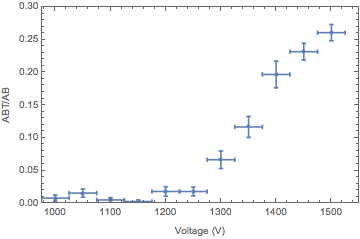
\includegraphics[width=8cm]{ABT.png}
\caption{Response curve of $A\cdot B\cdot T/ A\cdot B$}
\label{fig:ABT}
\end{figure}
\begin{figure}
\centering
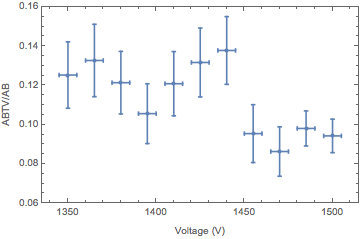
\includegraphics[width=8cm]{ABTV.png}
\caption{Response curve of $A\cdot B\cdot T \cdot \overline{V}/ A\cdot B$}
\label{fig:ABTV}
\end{figure}

Fitting the decay time histogram to an exponential, we obtain a first estimate of the muon lifetime. The fit is shown in figure~\ref{fig:fit}. To obtain a more accurate value, we plot the logarithm of the count totals and fit  The value of $\tau$ obtained from the slope of the linear fit is
\[
	\tau = \SI{2.125e-6}{s}.
\]
\begin{figure}
\centering
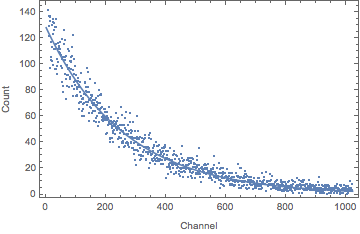
\includegraphics[width=8cm]{fit.png}
\caption{Exponential fit of decay time data}
\label{fig:fit}
\end{figure}

\begin{figure}
\centering
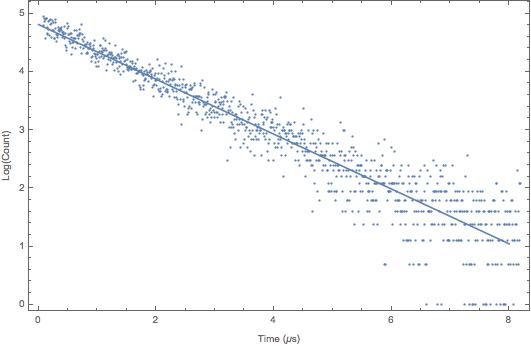
\includegraphics[width=8cm]{linearfit.png}
\caption{Linear fit of decay time data}
\label{fig:fit}
\end{figure}

We expect that not all of the events shown in figure~\ref{fig:fit} are from true muon decays. Since the TAC stops at any $A \cdot B$ signal, the TAC may be stopped prematurely due to background processes. However, we may use the measured $A \cdot B$ counting rate to remove some of this background and thus obtain a more precise measurement of the muon lifetime. By calculating the probability that in a given time interval $dt$ a false $A \cdot B$ signal will prematurely stop the TAC, we obtain a rough estimate of the number of false counts as a function of time. However, after completing this calculation, we determine that the effect of background is negligible and has no effect on our value of the muon lifetime. 

\section{Error}
We now determine a systematic error on our measurement of $e$. The standard error associated with the fitting parameter $\tau$ is calculated from Mathematica's LinearModelFit function. The value of $\sigma_{\tau}$ is given by
\[
	\sigma_{\tau} = \SI{0.0194}{\mu s}.
\]

\section{Conclusion}

We were able to calculate the value of $\tau$ to be
\[
    e = (2.217 \pm 0.0194) \times 10^{-6} \,\si{s}.
\]
Comparing this with the known value of the mean lifetime of the muon $\tau$, $\tau_0 = \SI{2.197e-6}{s}$, we see that $\tau_0$ falls within 2 standard deviations of our measurement.
Thus, our experimentally determined value of $\tau$ agrees reasonably with the
known value.
\end{document}
